The point \textbf{X} divides the line segment joining the two points \textbf{A}=\myvec{-1 \\ 1} and \textbf{B}=\myvec{5 \\ 7} in ratio k : 1. Then,\\
\begin{align}
\label{eq:solutions/line_plane_51/pointX}
\vec{X}=\frac{\brak{k\vec{B}+\vec{A}}}{\brak{k+1}}
\end{align}
From the equation \eqref{eq:solutions/line_plane_51/pointX}
\begin{align}
(k+1)\vec{X} = k\vec{B}+\vec{A}
\end{align}
Let \textbf{n}=\myvec{1\\1}
\begin{align}
\implies \brak{k+1}\vec{n}^T\vec{X}=\vec{n}^T\brak{k\vec{B}+\vec{A}}\\
\implies k\brak{\vec{n}^T\vec{X}-\vec{n}^T\vec{B}}=\vec{n}^T\vec{A}-\vec{n}^T\vec{X}
\end{align}
\begin{align}
\label{eq:solutions/line_plane_51/expk}
\implies k=\frac{\vec{n}^T\vec{A}-\vec{n}^T\vec{X}}{\vec{n}^T\vec{X}-\vec{n}^T\vec{B}}
\end{align}
Hence on solving the equation \eqref{eq:solutions/line_plane_51/expk} using
\begin{align}
\vec{n}^T\vec{X}=4
\end{align}
The line \myvec{1&1}\textbf{x}=4 divides the line joining points \textbf{A}=\myvec{-1\\1} and \textbf{B}=\myvec{5\\7} in the ratio k=1/2
See Fig. \ref{fig1:solutions/line_plane_51/}

\begin{figure}[!ht]
\centering
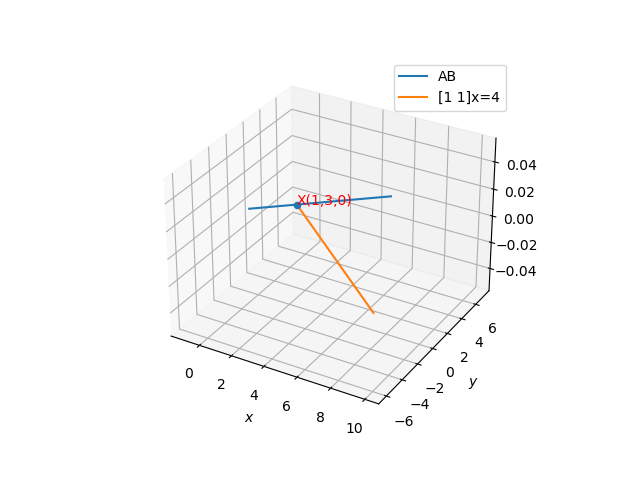
\includegraphics[width=\columnwidth]{./solutions/line_plane/51/Plot.png}
\caption{Line as (1 1)\textbf{x}=4 intersecting the line joining points A and B}
\label{fig1:solutions/line_plane_51/}
\end{figure}
